%==========================================================================
%Template File for Monthly Lectual Meeting
%2006/05/22 (kkobayashi@mikilab.doshisha.ac.jp)
%==========================================================================
\documentclass[a4j,9pt,twocolumn]{jsarticle}
\usepackage{mlm2.0}
\usepackage{epsf}
\pagestyle{plain}
\usepackage{url}
\usepackage{subfigure}
\setcounter{page}{1}
\usepackage{geometry}
\geometry{left=25mm,right=25mm,top=20mm,bottom=30mm}
%\usepackage[dvips]{graphicx}

\begin{document}
\twocolumn[
%---------------------------------------------------------------------------        % ヘッダ    書式:\beginheader{回}{年}{月}
%---------------------------------------------------------------------------
\beginheader{171}{2016}{04}
%---------------------------------------------------------------------------
% 発表題目    書式:\title{日本語}{英語} 「\\」で改行できます
%---------------------------------------------------------------------------
\title%
{git}%
%{更なる大容量化を目指して 進化しつづける次世代光メディア}

%---------------------------------------------------------------------------
% 著者名      書式:\author{日本語著者名}{英語著者名}
%---------------------------------------------------------------------------
\author{山下 俊樹,外村 篤紀\\Toshiki YAMASHITA,Atsuki TONOMURA}

%---------------------------------------------------------------------------
\endheader
%\begin{abstract}
%---------------------------------------------------------------------------
%Recently, a DVD attracts attention along with the image and the digitization of the sound. The standards of these DVD are complicated. So, in this paper, the standards of the DVD are summarized and the DVD of the next generation is refered. 
%---------------------------------------------------------------------------
%\end{abstract}
]

%---------------------------------------------------------------------------
% 本文
%---------------------------------------------------------------------------

\section{はじめに}
近年,ソフトウェアの大規模化にともない,プログラムの開発頻度は増加傾向にある.システムによる管理を行わず,開発に使用するファイルを編集した場合を考える.この場合,ファイルを以前の状態に復元したい時に,復元したい状態のファイルが発見しづらい問題点がある.そこで,コンピュータ上で作成または編集したファイルの変更履歴を管理するバージョン管理システムは,より重要となっている.本稿では,バージョン管理システムの1つであるgit,および関連サービスのGitHubについて述べる.

\section{git}
\subsection{概要}
gitはバージョン管理システムの1つであり,CUIで動作する.バージョン管理システムは,管理しているファイルを以前の状態に戻す機能や,複数人で1つのファイルを編集するときに発生してしまう競合を解消する機能を持つ.これらの機能を用いることで,開発中にバグが発生した場合,ファイルをバグが発生する以前の状態に復元できる利点がある\cite{pop}.

\subsection{構成}
gitで管理されるファイルやフォルダの変更内容は,リポジトリとよばれるデータベースに蓄積される.分散型バージョン管理システムにおけるリポジトリは2種類に分類できる.gitの構成を\fgref{git}に示す.

\begin{figure}[h]
\centering
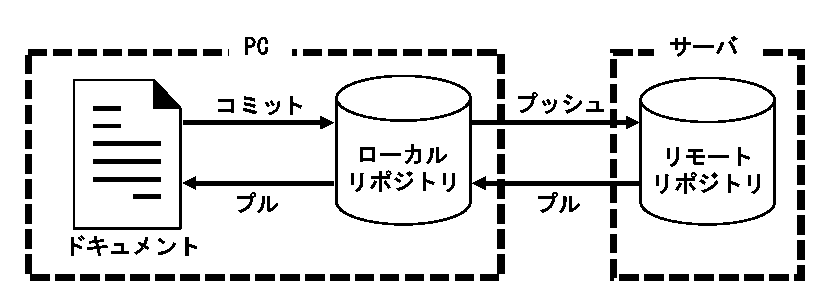
\includegraphics[width=80mm]{img/git.eps}
\caption{gitの構成}
\label{git}
\end{figure}

ローカルリポジトリは,個人のPC内に配置される.ファイルやフォルダの変更をローカルリポジトリに記録する操作をコミットとよぶ.コミットやプッシュを行うことで作業成果を記録する.ローカルリポジトリによって,ネットワークに接続されていない環境でもコミットを行うことができる.

リモートリポジトリは,サーバ上に配置され,複数ユーザで利用する.プルを行うことでリモートリポジトリから他者の作業成果をダウンロードしてローカルリポジトリに統合する.例えば,バグ修正のために個人のローカルリポジトリにコミットを行い,修正を完了したとする.その後,修正が完了したソフトウェアをリモートリポジトリにプッシュし,他者に公開する方法が可能である.

\subsection{バージョン管理}
gitは,履歴を管理するファイルを全て蓄積しており,必要なファイルを適切に取り出すことによりバージョン管理を実現している.バージョン管理の例を\fgref{tree}に示す.

\begin{figure}[h]
\centering
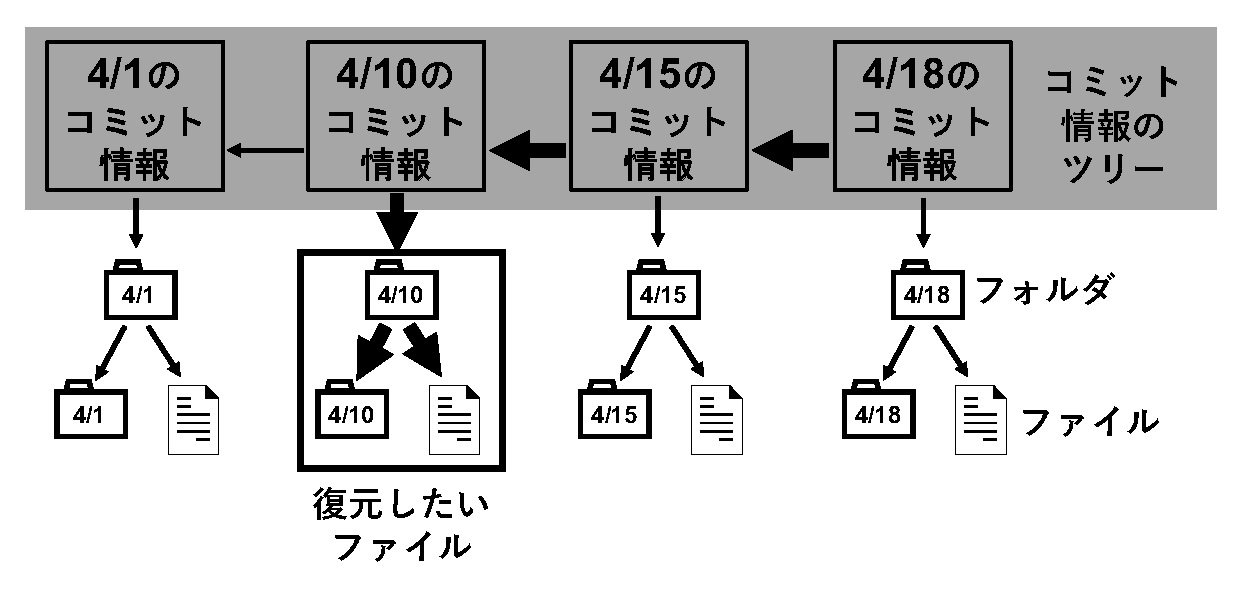
\includegraphics[width=85mm]{img/tree.eps}
\caption{バージョン管理の例}
\label{tree}
\end{figure}

コミットを行うと,コミット情報,および履歴を管理しているファイルがリポジトリに保存される.コミット情報は以下の2つで構成される.

\begin{itemize}
\item コミットしたファイルの保存場所
\item 前回のコミット情報の保存場所
\end{itemize}

前回のコミット情報の保存場所を辿ることで,復元したいファイルやフォルダにアクセスできる.

\subsection{ブランチ}
ブランチは,コミットの履歴の流れを分岐して管理することを指す.分岐したブランチ同士は互いに独立しており,異なる内容の更新を同時に行える.ブランチ同士の結合はマージとよぶ.ブランチを利用した例を\fgref{branch_ex}に示す.

\begin{figure}[h]
\centering
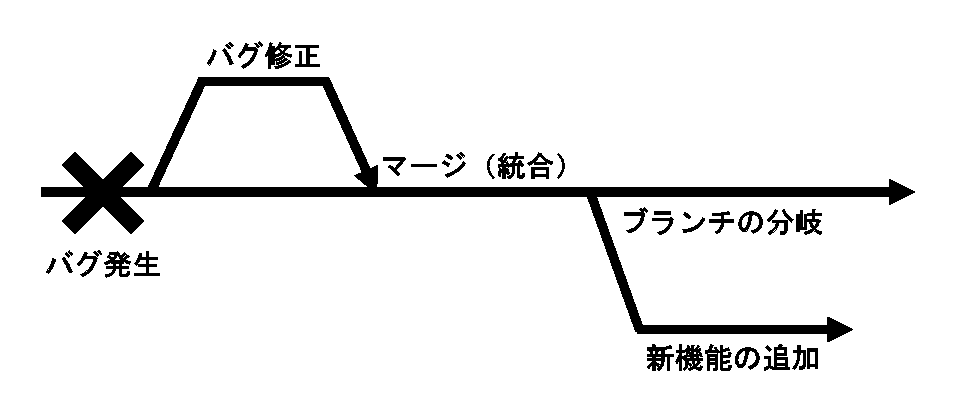
\includegraphics[width=90mm]{img/branch.eps}
\caption{ブランチの例}
\label{branch_ex}
\end{figure}

ブランチを用いることで,様々な開発やバグ修正などを並行して行うことができる.\fgref{branch_ex}において,既に運用されているソフトウェアの管理を行っているブランチを分岐する場合を考える.ソフトウェアのバグ修正や,新機能を追加するために,それぞれブランチを分岐する.この場合,3つのブランチは独立しているため,運用中のソフトウェアに影響を与えることなく,バグ修正と新機能の追加を行える.ブランチを用いない場合,修正や開発を行うためには,ソフトウェアの運用を停止しなければならない.しかし,ブランチを用いることで,ソフトウェアの運用を継続しながら,他の修正や開発を行うことができる.

gitのブランチは,他のバージョン管理システムに比べて優れている.他のシステムでは,マージの際にどのファイルをどのようにマージするか入力する必要があるが,gitは自動的に行うことができる.管理するファイルが多い場合,手動でマージの指示を入力するには労力を要する.しかし,gitを用いることでマージが自動的に行われ,労力を削減できる.

\section{GitHub}
\subsection{概要}
GitHubとは,gitを利用したSNSである.現在,GitHubは最も人気のあるgitサービス提供サイトであり,そのユーザ数は1000万人を超えている\cite{github}.GitHubの特徴の1つは,分かりやすいGUIである.GitHubのリモートリポジトリの内容は全て公開されるため,ソースコードを公開できないWebデザインや,個人情報を扱う開発などには利用できない.しかし,リモートリポジトリが無料で提供されるため,個人でリモートリポジトリ用のサーバを用意する必要がない.その結果,GitHubは手軽にリモートリポジトリを使用できるサービスとして広まった.

他のユーザと協力してソースコードを管理するための機能として,コードレビュー,およびコメント機能がある.コードレビューとは,ソースコードに含まれる誤りを検出,修正することを目的として行われるソースコードの査読を指す.これらの機能を用いることで,各ユーザが互いのソースコードを評価することができる.その結果,ソースコードの改善が行われ,ソースコードのバグの解消や可読性の向上といった利点を生む.

\subsection{GitHubにおけるブランチの活用例}
gitのブランチの分岐は,GitHubではフォークとよばれる.GitHubのユーザは他のユーザのリポジトリからフォークしたアプリケーションを引き継いで開発することができる.フォークに1つのタスクを割り当てることでチケット駆動開発を行うことができる.

次に,チケットについて述べる.チケットとは,全体の作業を細かいタスクに分割し,タスク1つ1つに対して割り振られる,各タスクの作業指示である.開発者は発行されたチケットを取り,チケットに記されたタスク(バグ修正や機能追加など)をこなす.指示内容が完了するとコミットを行い,チケットを消去(クローズ)する.タスクをチケットで管理することにより,作業の全容が把握しやすいことや,チーム開発においてタスクの分配が行いやすくなる利点がある.

\begin{figure}[h]
\centering
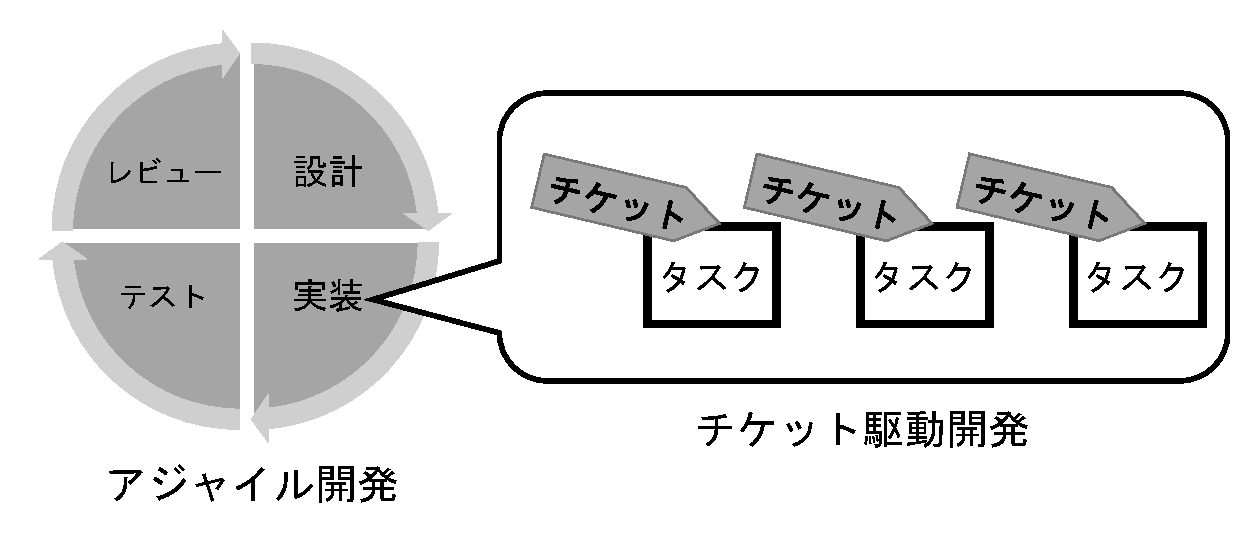
\includegraphics[width=80mm]{img/dev.eps}
\caption{アジャイル開発とチケット駆動開発}
\label{dev}
\end{figure}

チケットを用いて行うチケット駆動開発は,アジャイル開発とも親和性が高い.アジャイル開発とは,開発対象を多数の小さな機能に分割し,短い期間(1週間から4週間)で1つの機能を開発する工程を反復しながら,開発を行う手法である.アジャイル開発における小さな機能は,チケット駆動開発のタスクに対応する.\fgref{branch_ex}に示したように,アジャイル開発におけるタスクにチケットを割り当てることで,チケット駆動開発との統合を実現する.チケット駆動開発を行う際には,オンラインプロジェクト管理ソフトウェアであるRedmineを併用する場合が多い.

\subsection{BitBucketとの比較}
GitHubに競合するサービスとして,BitBucketが挙げられる. GitHubに対して,無料で非公開のリモートリポジトリを作成できる利点があるが,1つのリモートリポジトリを利用できるユーザ数は最大5人に限られる.そのため,ソースコードを共有して開発を行える人数が5人に限られる.その結果,大人数での開発には使用できず,開発規模が制限される欠点がある.

どちらのサービスもソーシャルコーディングの普及に貢献しているが,現時点でのユーザ数はGitHubが圧倒的に多い.これは,GitHubに対応する周辺サービスが多いこと,著名な開発プロジェクトが多数あること,およびGUIが使いやすいことによる.

\section{今後の展望}
今日,ソフトウェアのリリース速度は増加の一途を辿っている.それにともない,開発の効率化,高速化が重要視されている.そのため,gitのようなバージョン管理ソフトウェアは更に普及すると考えられる.また,GitHubのようなgitを用いたサービスは,現在概ね無料で公開されている.しかし,ソフトウェアの開発において,デバッグや開発の一部を他者に依頼し,一番良いソースコードを含むフォークに報酬を払うビジネスといった,商業利用が近い将来に生まれると考える.

\small
\begin{thebibliography}{99}
\bibitem{pop}
岡本隆史:Gitに潜む光と闇,入手先,(http://gihyo.jp/dev/column/01/prog/2012/git)

\bibitem{mecha}
koseki2:Git の仕組み (1),入手先(http://koseki.\\hatenablog.com/entry/2014/04/22/inside-git-1)

\bibitem{github}
Ken Nishimura,市民生活をオープンデータ活用で改善する政府や地域行政の事例 [GitHub Universe],(http://thebridge.jp/2015/10/github-universe-session-changing-lives-with-open-data).
\end{thebibliography}
\end{document}